\documentclass{ximera}
\graphicspath{  %% When looking for images,
{./}            %% look here first,
{./pictures/}   %% then look for a pictures folder,
{../pictures/}  %% which may be a directory up.
{../../pictures/}  %% which may be a directory up.
{../../../pictures/}  %% which may be a directory up.
{../../../../pictures/}  %% which may be a directory up.
}

\usepackage{listings}
\usepackage{circuitikz}
\usepackage{xcolor}
\usepackage{amsmath,amsthm}
\usepackage{subcaption}
\usepackage{graphicx}
\usepackage{tikz}
\usepackage{tikz-3dplot}
\usepackage{amsfonts}
\usepackage{mdframed} % For framing content
\usepackage{tikz-cd}

  \renewcommand{\vector}[1]{\left\langle #1\right\rangle}
  \newcommand{\arrowvec}[1]{{\overset{\rightharpoonup}{#1}}}
  \newcommand{\ro}{\texttt{R}}%% row operation
  \newcommand{\dotp}{\bullet}%% dot product
  \renewcommand{\l}{\ell}
  \let\defaultAnswerFormat\answerFormatBoxed
  \usetikzlibrary{calc,bending}
  \tikzset{>=stealth}
  




%make a maroon color
\definecolor{maroon}{RGB}{128,0,0}
%make a dark blue color
\definecolor{darkblue}{RGB}{0,0,139}
%define the color fourier0 to be the maroon color
\definecolor{fourier0}{RGB}{128,0,0}
%define the color fourier1 to be the dark blue color
\definecolor{fourier1}{RGB}{0,0,139}
%define the color fourier 1t to be the light blue color
\definecolor{fourier1t}{RGB}{173,216,230}
%define the color fourier2 to be the dark green color
\definecolor{fourier2}{RGB}{0,100,0}
%define teh color fourier2t to be the light green color
\definecolor{fourier2t}{RGB}{144,238,144}
%define the color fourier3 to be the dark purple color
\definecolor{fourier3}{RGB}{128,0,128}
%define the color fourier3t to be the light purple color
\definecolor{fourier3t}{RGB}{221,160,221}
%define the color fourier0t to be the red color
\definecolor{fourier0t}{RGB}{255,0,0}
%define the color fourier4 to be the orange color
\definecolor{fourier4}{RGB}{255,165,0}
%define the color fourier4t to be the darker orange color
\definecolor{fourier4t}{RGB}{255,215,0}
%define the color fourier5 to be the yellow color
\definecolor{fourier5}{RGB}{255,255,0}
%define the color fourier5t to be the darker yellow color
\definecolor{fourier5t}{RGB}{255,255,100}
%define the color fourier6 to be the green color
\definecolor{fourier6}{RGB}{0,128,0}
%define the color fourier6t to be the darker green color
\definecolor{fourier6t}{RGB}{0,255,0}

%New commands for this doc for errors in copying
\newcommand{\eigenvar}{\lambda}
%\newcommand{\vect}[1]{\mathbf{#1}}
\renewcommand{\th}{^{\text{th}}}
\newcommand{\st}{^{\text{st}}}
\newcommand{\nd}{^{\text{nd}}}
\newcommand{\rd}{^{\text{rd}}}
\newcommand{\paren}[1]{\left(#1\right)}
\newcommand{\abs}[1]{\left|#1\right|}
\newcommand{\R}{\mathbb{R}}
\newcommand{\C}{\mathbb{C}}
\newcommand{\Hilb}{\mathbb{H}}
\newcommand{\qq}[1]{\text{#1}}
\newcommand{\Z}{\mathbb{Z}}
\newcommand{\N}{\mathbb{N}}
\newcommand{\q}[1]{\text{``#1''}}
%\newcommand{\mat}[1]{\begin{bmatrix}#1\end{bmatrix}}
\newcommand{\rref}{\text{reduced row echelon form}}
\newcommand{\ef}{\text{echelon form}}
\newcommand{\ohm}{\Omega}
\newcommand{\volt}{\text{V}}
\newcommand{\amp}{\text{A}}
\newcommand{\Seq}{\textbf{Seq}}
\newcommand{\Poly}{\textbf{P}}
\renewcommand{\quad}{\text{    }}
\newcommand{\roweq}{\simeq}
\newcommand{\rowop}{\simeq}
\newcommand{\rowswap}{\leftrightarrow}
\newcommand{\Mat}{\textbf{M}}
\newcommand{\Func}{\textbf{Func}}
\newcommand{\Hw}{\textbf{Hamming weight}}
\newcommand{\Hd}{\textbf{Hamming distance}}
\newcommand{\rank}{\text{rank}}
\newcommand{\longvect}[1]{\overrightarrow{#1}}
% Define the circled command
\newcommand{\circled}[1]{%
  \tikz[baseline=(char.base)]{
    \node[shape=circle,draw,inner sep=2pt,red,fill=red!20,text=black] (char) {#1};}%
}

% Define custom command \strikeh that just puts red text on the 2nd argument
\newcommand{\strikeh}[2]{\textcolor{red}{#2}}

% Define custom command \strikev that just puts red text on the 2nd argument
\newcommand{\strikev}[2]{\textcolor{red}{#2}}

%more new commands for this doc for errors in copying
\newcommand{\SI}{\text{SI}}
\newcommand{\kg}{\text{kg}}
\newcommand{\m}{\text{m}}
\newcommand{\s}{\text{s}}
\newcommand{\norm}[1]{\left\|#1\right\|}
\newcommand{\col}{\text{col}}
\newcommand{\sspan}{\text{span}}
\newcommand{\proj}{\text{proj}}
\newcommand{\set}[1]{\left\{#1\right\}}
\newcommand{\degC}{^\circ\text{C}}
\newcommand{\centroid}[1]{\overline{#1}}
\newcommand{\dotprod}{\boldsymbol{\cdot}}
%\newcommand{\coord}[1]{\begin{bmatrix}#1\end{bmatrix}}
\newcommand{\iprod}[1]{\langle #1 \rangle}
\newcommand{\adjoint}{^{*}}
\newcommand{\conjugate}[1]{\overline{#1}}
\newcommand{\eigenvarA}{\lambda}
\newcommand{\eigenvarB}{\mu}
\newcommand{\orth}{\perp}
\newcommand{\bigbracket}[1]{\left[#1\right]}
\newcommand{\textiff}{\text{ if and only if }}
\newcommand{\adj}{\text{adj}}
\newcommand{\ijth}{\emph{ij}^\text{th}}
\newcommand{\minor}[2]{M_{#2}}
\newcommand{\cofactor}{\text{C}}
\newcommand{\shift}{\textbf{shift}}
\newcommand{\startmat}[1]{
  \left[\begin{array}{#1}
}
\newcommand{\stopmat}{\end{array}\right]}
%a command to give a name to explorations and hints and theorems
\newcommand{\name}[1]{\begin{centering}\textbf{#1}\end{centering}}
\newcommand{\vect}[1]{\vec{#1}}
\newcommand{\dfn}[1]{\textbf{#1}}
\newcommand{\transpose}{\mathsf{T}}
\newcommand{\mtlb}[2][black]{\texttt{\textcolor{#1}{#2}}}
\newcommand{\RR}{\mathbb{R}} % Real numbers
\newcommand{\id}{\text{id}}

\author{Zack Reed}
%borrowed from selinger linear algebra
\title{Vector Subspaces: Lines and Planes - Lines}
\begin{document}
\begin{abstract}

    This covers lines

\end{abstract}
\maketitle



\section{Lines}

%\begin{outcome}
  \begin{enumerate}
  \item Find the vector, parametric, and symmetric equations of a line.
  \item Determine whether a point is on a given line.
  \item Determine whether two lines intersect.
  \item Find the angle between two lines.
  \item Find the projection of a point onto a line.
  \end{enumerate}
%\end{outcome}

We can use the concept of vectors and points to find equations for
lines in $\R^n$. Consider a straight line $L$ that passes through a
point $P$ in the direction given by a non-zero vector $\vect{d}$.
\begin{center}
  \begin{tikzpicture}[rotate=10]
    % Note: I deliberately made the red a bit lighter and the blue a bit
    % darker, so that it will also look okay in black-and-white.
    \draw[red!80](-4,0) -- node [above=3pt, pos=0.875] {$L$} (9,0);
    \draw[->,thick,blue!80!black](0,0) -- node[above left] {$\vect{d}$} (2,0);
    \fill (0,0) circle [radius=2.2pt] node [above=3pt] {$P$};
    \fill (5,0) circle [radius=2.2pt] node [above=3pt] {$Q$};
  \end{tikzpicture}
\end{center}
The line $L$ is infinitely long in both directions, although the
picture only shows a finite part of it. To find an equation for this
line, first suppose that $Q$ is an arbitrary point on $L$. Then the
vector $\longvect{PQ}$ is parallel to $\vect{d}$. In other words,
there exists some real number $t$ such that
\begin{equation*}
  \longvect{PQ} = t\,\vect{d}.
\end{equation*}
If $\vect{p}$ is the position vector of $P$ and $\vect{q}$ is the
position vector of $Q$, we can write
\begin{equation*}
  \longvect{PQ} = \vect{q}-\vect{p}.
\end{equation*}
Putting together the last two equations, we get $\vect{q}-\vect{p} =
t\,\vect{d}$, which we can write as
\begin{equation*}
  \vect{q} = \vect{p} + t\,\vect{d}.
\end{equation*}
This is called the \textbf{vector equation}%
\index{vector equation!of a line}%
\index{line!vector equation} of the line $L$. The vector $\vect{d}$ is
called the \textbf{direction vector}%
\index{direction vector}%
\index{vector!direction vector}, and $t$ is called a
\textbf{parameter}%
\index{parameter}. The parameter $t$ can be any real number; each time
we plug in a different number for $t$, we get a different point $Q$ on
the line. The following picture shows the effect of the parameter:
\begin{center}
  \begin{tikzpicture}[rotate=10]
    % Note: I deliberately made the red a bit lighter and the blue a bit
    % darker, so that it will also look okay in black-and-white.
    \draw[red!80](-4,0) -- node [above=3pt, pos=0.92] {$L$} (10,0);
    \draw[->,thick,blue!80!black](0,0) -- node[above=3pt] {$\vect{d}$} (2,0);
    \draw[->,thick,blue!80!black](3,-2) -- node[below=3pt] {$\vect{p}$} (0,0);
    \fill (0,0) circle [radius=2.2pt] node [above=3pt] {$P$};
    \fill (-2,0) circle [radius=2.2pt] node [below=9pt] {$t=-1$};
    \fill (0,0) circle [radius=2.2pt] node [below=10pt] {$t=0$};
    \fill (2,0) circle [radius=2.2pt] node [below=10pt] {$t=1$};
    \fill (4,0) circle [radius=2.2pt] node [below=10pt] {$t=2$};
    \fill (6,0) circle [radius=2.2pt] node [below=10pt] {$t=3$};
    \fill (8,0) circle [radius=2.2pt] node [below=10pt] {$t=3$};
    \fill (3,-2) circle [radius=2.2pt] node [right=3pt] {$0$};
  \end{tikzpicture}
\end{center}
The following definition summarizes the above.

\begin{definition}{Vector equation of a line}{vector-equation-of-line}
  Let $\vect{p}$ be a vector and $\vect{d}$ a non-zero vector. Then
  \begin{equation*}
    \vect{q} = \vect{p} + t\,\vect{d}
  \end{equation*}
  is the \textbf{vector equation}%
  \index{vector equation!of a line}%
  \index{line!vector equation} of a straight line $L$. Specifically,
  as the parameter $t$ ranges over the real numbers, $\vect{q}$ ranges
  over the position vectors of all the points $Q$ on the line $L$.
  The vector $\vect{d}$ is called the \textbf{direction vector}%
  \index{direction vector}%
  \index{vector!direction vector} of the line.
\end{definition}

\begin{example}{A line from a point and a direction vector}{line-point-and-direction-vector}
  Find a vector equation for the line which contains the point
  $P = (2,0,3)$ and has direction vector
  $\vect{d} = \startmat{c}1,2,1\stopmat^T$.
\end{example}

\begin{solution}
  The position vector of the point $P$ is
  $\vect{p}=\startmat{c}2,0,3\stopmat^T$. The equation of the line is
  $\vect{q}= \vect{p} + t\,\vect{d}$, which we can write as
  \begin{equation*}
    \startmat{c} x \\ y \\ z \stopmat
    = \startmat{c} 2 \\ 0 \\ 3 \stopmat
    + t \startmat{c} 1 \\ 2 \\ 1 \stopmat.
  \end{equation*}
\end{solution}

\begin{example}{A line from two points}{line-from-two-points}
  Find a vector equation for the line through the points
  $P = (1,2,0,1)$ and $R = (2,-4,6,3)$.
\end{example}

\begin{solution}
  We can use $P$ as the base point; its position vector is
  $\vect{p}=\startmat{c}1,2,0,1\stopmat^T$. We can use
  $\vect{d}=\longvect{PR}=\startmat{c}1,-6,6,2\stopmat$ as the direction vector. Then
  a vector equation of the line is
  $\vect{q} = \vect{p} + t\,\vect{d}$,
  which we can also write as
  \begin{equation*}
    \startmat{c} x \\ y \\ z \\ w \stopmat
    = \startmat{c} 1 \\ 2 \\ 0 \\ 1\stopmat
    + t \startmat{r} 1 \\ -6 \\ 6 \\ 2\stopmat.
  \end{equation*}
\end{solution}

When we write a vector equation in the form
\begin{equation*}
  \startmat{c} x_1 \\ x_2 \\ \vdots \\ x_n \stopmat
  = \startmat{c} p_1 \\ p_2 \\ \vdots \\ p_n \stopmat
  + t \startmat{r} d_1 \\ d_2 \\ \vdots \\ d_n \stopmat,
\end{equation*}
it is also called the \textbf{component form}%
\index{vector equation!of a line!component form}%
\index{component form!line}%
\index{line!component form} of the vector equation.

Notice that the vector equation of a line is not unique. In fact,
there are infinitely many vector equations for the same line. For
example, we can replace the parameter $t$ with another parameter, say
$3s$ or $1-r$.

\begin{example}{Change of parameter}{change-of-parameter}
  Consider the vector equation from
  Example~\ref{exa:line-point-and-direction-vector},
  \begin{equation*}
    \startmat{c} x \\ y \\ z \stopmat
    = \startmat{c} 2 \\ 0 \\ 3 \stopmat
    + t \startmat{c} 1 \\ 2 \\ 1 \stopmat.
  \end{equation*}
  Find two other equations for the same line, by changing the
  parameter%
  \index{line!change of parameter}%
  \index{change of parameters!line} to $3s$ and to $1-r$.
\end{example}

\begin{solution}
  If we let $t=3s$, we get
  \begin{equation*}
    \begin{array}{rcl}
      \startmat{c} x \\ y \\ z \stopmat
      &=& \startmat{c} 2 \\ 0 \\ 3 \stopmat
      + 3s \startmat{c} 1 \\ 2 \\ 1 \stopmat\\\\[-1ex]
      &=& \startmat{c} 2 \\ 0 \\ 3 \stopmat
      + s \startmat{c} 3 \\ 6 \\ 3 \stopmat.
    \end{array}
  \end{equation*}
  If we let $t=1-r$, we get
  \begin{equation*}
    \begin{array}{rcl}
      \startmat{c} x \\ y \\ z \stopmat
      &=& \startmat{c} 2 \\ 0 \\ 3 \stopmat
      + (1-r) \startmat{c} 1 \\ 2 \\ 1 \stopmat\\\\[-1ex]
      &=& \startmat{c} 2 \\ 0 \\ 3 \stopmat
      + \startmat{c} 1 \\ 2 \\ 1 \stopmat
      - r \startmat{c} 1 \\ 2 \\ 1 \stopmat\\\\[-1ex]
      &=& \startmat{c} 3 \\ 2 \\ 4 \stopmat
      + r \startmat{c} -1 \\ -2 \\ -1 \stopmat.
    \end{array}
  \end{equation*}
\end{solution}

\begin{definition}{Parametric equations of a line}{parametric-equations}
  A line with vector equation
  \begin{equation*}
    \startmat{c} x_1 \\ x_2 \\ \vdots \\ x_n \stopmat
    = \startmat{c} p_1 \\ p_2 \\ \vdots \\ p_n \stopmat
    + t \startmat{r} d_1 \\ d_2 \\ \vdots \\ d_n \stopmat
  \end{equation*}
  can also be written as a set of $n$ scalar equations:
  \begin{equation*}
    \begin{array}{c@{~}c@{~}c}
      x_1 &=& p_1 + t\,d_1, \\
      x_2 &=& p_2 + t\,d_2, \\
          &\vdots&             \\
      x_n &=& p_n + t\,d_n,
    \end{array}
  \end{equation*}
  When written in this form, they are called the \textbf{parametric
    equations}%
  \index{parametric equations!of a line}%
  \index{line!parametric equations} of the line.
\end{definition}

\begin{example}{Parametric equations}{parametric-equation}
  Find parametric equations for the line through the points
  $P = (1,2,0,1)$ and $R = (2,-4,6,3)$.
\end{example}

\begin{solution}
  This is a same line as in Example~\ref{exa:line-from-two-points}. We
  can easily convert the vector equation
  \begin{equation*}
    \startmat{c} x \\ y \\ z \\ w \stopmat
    = \startmat{c} 1 \\ 2 \\ 0 \\ 1\stopmat
    + t \startmat{r} 1 \\ -6 \\ 6 \\ 2\stopmat
  \end{equation*}
  to a set of parametric equations:
  \begin{equation*}
    \begin{array}{c@{~}c@{~}l}
      x &=& 1 + t, \\
      y &=& 2 - 6t, \\
      z &=& 6t, \\
      w &=& 1 + 2t.
    \end{array}
  \end{equation*}
\end{solution}

\begin{example}{Determine whether a point is on a line}{point-on-line}
  Determine whether the point $P=(5,8,4)$ is on the line $L$ given by
  the vector equation
  \begin{equation*}
    \startmat{c} x \\ y \\ z \stopmat
    = \startmat{c} 1 \\ 2 \\ 1 \stopmat
    + t \startmat{c} 2 \\ 3 \\ 1 \stopmat.
  \end{equation*}
\end{example}

\begin{solution}
  The point $P$ is on the line $L$ if and only if there exists some
  $t\in\R$ such that
  \begin{equation*}
    \startmat{c} 1 \\ 2 \\ 1 \stopmat
    + t \startmat{c} 2 \\ 3 \\ 1 \stopmat
    = \startmat{c} 5 \\ 8 \\ 4 \stopmat.
  \end{equation*}
  Subtracting $\startmat{c}1,2,1\stopmat^T$ from both sides of the equation, this is
  equivalent to
  \begin{equation*}
    t \startmat{c} 2 \\ 3 \\ 1 \stopmat
    = \startmat{c} 4 \\ 6 \\ 3 \stopmat.
  \end{equation*}
  We can write this as a set of parametric equations:
  \begin{equation*}
    \begin{array}{c@{~}c@{~}l}
      2t &=& 4, \\
      3t &=& 6, \\
      t &=& 3.
    \end{array}
  \end{equation*}
  This is a system of three linear equations in one variable, and we
  quickly see that it is inconsistent. Therefore, the point $P$ does
  not lie on the line $L$.
\end{solution}

\begin{example}{Determine whether two lines intersect}{lines-intersect}
  Determine whether the lines
  \begin{equation*}
    \startmat{c} x \\ y \\ z \stopmat
    = \startmat{c} 3 \\ 1 \\ 0 \stopmat
    + t \startmat{c} 2 \\ 0 \\ 1 \stopmat
    \quad\mbox{and}\quad
    \startmat{c} x \\ y \\ z \stopmat
    = \startmat{c} 1 \\ -1 \\ 5 \stopmat
    + s \startmat{c} 2 \\ 1 \\ -2 \stopmat
  \end{equation*}
  intersect. If yes, find the point of intersection.%
  \index{intersection!of two lines}
\end{example}

\begin{solution}
  The two lines intersect if and only if there exist $t,s\in\R$ such
  that
  \begin{equation*}
    \startmat{c} 3 \\ 1 \\ 0 \stopmat
    + t \startmat{c} 2 \\ 0 \\ 1 \stopmat
    = \startmat{c} 1 \\ -1 \\ 5 \stopmat
    + s \startmat{c} 2 \\ 1 \\ -2 \stopmat.
  \end{equation*}
  Bringing $s$ to the left-hand side, and subtracting $\startmat{c}3,1,0\stopmat^T$
  from both sides of the equation, this is equivalent to
  \begin{equation*}
    t \startmat{c} 2 \\ 0 \\ 1 \stopmat
    - s \startmat{c} 2 \\ 1 \\ -2 \stopmat
    = \startmat{c} -2 \\ -2 \\ 5 \stopmat.
  \end{equation*}
  If we write this vector equation as a set of three parametric
  equations, it is a system of 3 linear equations in 2 variables. The
  augmented matrix of the system is
  \begin{equation*}
    \startmat{cc|c}
      2 & -2 & -2 \\
      0 & -1 & -2 \\
      1 & 2 & 5   \\
    \stopmat.
  \end{equation*}
  This system has {\rref}
  \begin{equation*}
    \startmat{cc|c}
      1 & 0 & 1 \\
      0 & 1 & 2 \\
      0 & 0 & 0 \\
    \stopmat,
  \end{equation*}
  and has the unique solution $t=1$ and $s=2$. Therefore, the lines
  intersect. (Other possible cases are: If the system is inconsistent,
  the lines do not intersect. If the system has more than one
  solution, the lines are identical). We find the point of
  intersection by plugging the parameter $t=1$ into the equation of
  the first line (or equivalently, but plugging $s=2$ into the
  equation of the second line - doing it both ways is a good way to
  double-check your answer). Therefore, the point of intersection is
  \begin{equation*}
    \startmat{c} 3 \\ 1 \\ 0 \stopmat
    + 1 \startmat{c} 2 \\ 0 \\ 1 \stopmat
    = \startmat{c} 5 \\ 1 \\ 1 \stopmat.
  \end{equation*}
\end{solution}

There is one other form for a line which is useful, which is the
\textbf{symmetric form}.  Consider the line given by
\begin{equation*}
  \begin{array}{c@{~}c@{~}l}
    x &=& 1 + 2t, \\
    y &=& 1 - t, \\
    z &=& 3 + 2t. \\
  \end{array}
\end{equation*}
We can solve each equation for $t$:
\begin{equation*}
  \begin{array}{c@{~}c@{~}l}
    t &=& \frac{x-1}{2}, \\\\[-2ex]
    t &=& \frac{y-1}{-1}, \\\\[-2ex]
    t &=& \frac{z-3}{2}.
  \end{array}
\end{equation*}
Finally, we can eliminate $t$ from the equations by setting all three
equations equal to one another:
\begin{equation*}
  \frac{x-1}{2} = \frac{y-1}{-1} = \frac{z-3}{2}.
\end{equation*}
The latter is really a system of 2 equations in 3 variables.  This is
the \textbf{symmetric form}%
\index{line!symmetric form equation}%
\index{symmetric form} of the equation of the line.  In the following
example, we look at how to convert the equation of a line from
symmetric form to parametric form.

\begin{example}{Change symmetric form to parametric form}{symmetric-to-parametric}
  Consider the line whose equations are given in \textbf{symmetric form} as
  \begin{equation*}
    \frac{x-2}{3}=\frac{y-1}{2}=\frac{z+3}{1}.
  \end{equation*}
  Find parametric and vector equations for this line.
\end{example}

\begin{solution}
  We set all three quantities equal to $t$:
  \begin{equation*}
    t=\frac{x-2}{3}, \quad
    t=\frac{y-1}{2}, \quad
    t=\frac{z+3}{1}.
  \end{equation*}
  Solving these equations for $x,y,z$ yields
  \begin{equation*}
    \begin{array}{c}
      x = 2 + 3t, \\
      y = 1 + 2t, \\
      z = -3 + t.
    \end{array}
  \end{equation*}
  These are the parametric equations for the line. The vector equation
  is
  \begin{equation*}
    \startmat{c}
      x \\
      y \\
      z
    \stopmat =
    \startmat{r}
      2 \\
      1 \\
      -3
    \stopmat
    +
    t
    \startmat{r}
      3 \\
      2 \\
      1
    \stopmat.
  \end{equation*}
\end{solution}

We can use the dot product to find the angle between two intersecting
lines. This is simply the smallest angle between (any of) their
direction vectors. The only subtlety here is that if $\vect{u}$ is a
direction vector for a line, then so is $-\vect{u}$, and thus we will
find pairs of complementary angles. We will take the smaller of the
two angles.
\begin{center} 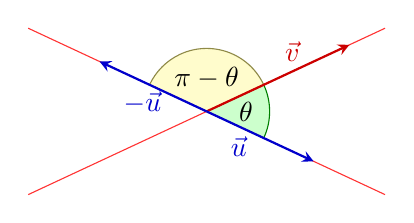
\begin{tikzpicture}
    \filldraw[fill=green!20,draw=green!50!black] (0,0) -- (-25:8mm)
    arc (-25:25:8mm) -- cycle;
    \filldraw[fill=yellow!20,draw=yellow!50!black] (0,0) -- (25:8mm)
    arc (25:155:8mm) -- cycle;
    \node at (0:5mm) {$\theta$};
    \node at (90:4.2mm) {$\pi-\theta$};
    \draw[red!80](25:-2.5) -- (25:2.5);
    \draw[red!80](-25:-2.5) -- (-25:2.5);
    \draw[->,thick,red!80!black](0,0) -- node[above,pos=0.6]{$\vect{v}$} (25:2);
    \draw[->,thick,blue!80!black](0,0) -- node[below,pos=0.3]{$\vect{u}$} (-25:1.5);
    \draw[->,thick,blue!80!black](0,0) -- node[below,pos=0.6]{$-\vect{u}$} (155:1.5);
  \end{tikzpicture}
\end{center}

\begin{example}{Find the angle between two lines}{angle-between-two-lines}
  Find the angle between the two lines%
  \index{line!angle between}%
  \index{angle!between two lines}
  \begin{equation*}
    L_1:  \;
    \startmat{r} x \\ y \\ z \stopmat
    = \startmat{r} 1 \\ 2 \\ 0 \stopmat
    + t \startmat{r} -1 \\ 1 \\ 2 \stopmat
  \end{equation*}
  and
  \begin{equation*}
    L_2: \;
    \startmat{r} x \\ y \\ z \stopmat
    = \startmat{r} 0 \\ 3 \\ 2 \stopmat
    + s \startmat{r} 2 \\ 1 \\ -1 \stopmat.
  \end{equation*}
\end{example}

\begin{solution}
  The direction vectors are
  \begin{equation*}
    \vect{u}=\startmat{r} -1 \\ 1 \\ 2 \stopmat
    \quad\mbox{and}\quad
    \vect{v}=\startmat{r} 2 \\ 1 \\ -1 \stopmat.
  \end{equation*}
  The answer is given by
  \begin{equation*}
    \cos\theta =
    \frac{\vect{u}\dotprod\vect{v}}{\norm{\vect{u}}\norm{\vect{v}}} = -\frac{1}{2},
  \end{equation*}
  which gives $\theta=\frac{2\pi}{3}$.  Now the angles between any two
  direction vectors for these lines will either be $\frac{2 \pi}{3}$ or
  its complement $\phi = \pi - \frac{2 \pi}{3} = \frac{\pi}{3}$. We
  choose the smaller angle, and therefore conclude that the angle
  between the two lines is $\frac{\pi}{3}$.
\end{solution}



Finally, we will show how to use projections to find the shortest
distance from a point to a line.

\begin{example}{Shortest distance from a point to a line}
  Let $L$ be the line which goes through the point $P = (0,4,-2)$ with
  direction vector
  $\vect{d} = \startmat{r} 2 \\ 1 \\
    2 \stopmat$, and let $Q=(1,3,5)$. Find the shortest
  distance%
  \index{distance!point to line} from $Q$ to the line $L$, and find
  the point $R$ on $L$ that is closest to $Q$.%
  \index{projection!point to line}
  \begin{center}
    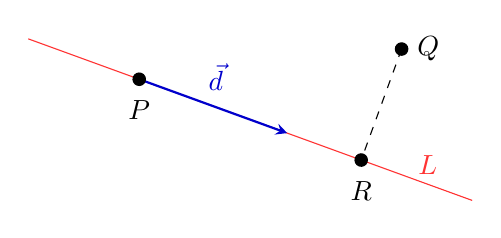
\begin{tikzpicture}[rotate=-20]
      \draw[red!80](-1.5,0) -- node[above, pos=0.9]{$L$} (4.5,0);
      \draw[->,thick,blue!80!black](0,0) -- node[above right, pos=0.4]{$\vect{d}$} (2,0);
      \draw[dashed] (3,1.5) -- (3,0);
      \draw[fill](0,0) circle [radius=2.25pt] node[below=1ex]{$P$};
      \draw[fill](3,1.5) circle [radius=2.25pt] node[right=0.5ex]{$Q$};
      \draw[fill](3,0) circle [radius=2.25pt] node[below=1ex]{$R$};
    \end{tikzpicture}
  \end{center}
\end{example}

\end{document}

\begin{solution}
  In order to determine the shortest distance from $Q$ to $L$, we will
  first find the vector $\longvect{PQ}$ and then find the projection
  of this vector onto $L$.  The vector $\longvect{PQ}$ is given by
  \begin{equation*}
    \longvect{PQ}=
    \startmat{r} 1 \\ 3 \\ 5 \stopmat
    - \startmat{r} 0 \\ 4 \\ -2 \stopmat
    = \startmat{r} 1 \\ -1 \\ 7 \stopmat.
  \end{equation*}
  Then, if $R$ is the point on $L$ closest to $Q$, it follows that
  \begin{equation*}
    \longvect{PR}
    ~=~ \proj_{\vect{d}}\longvect{PQ} \\
    ~=~ \frac{\vect{d}\dotprod\longvect{PQ}}{\norm{\vect{d}}^2}\,\vect{d} \\
    ~=~ \frac{15}{9} \startmat{r} 2 \\ 1 \\ 2 \stopmat \\
    ~=~ \frac{5}{3} \startmat{r} 2 \\ 1 \\ 2 \stopmat.
  \end{equation*}
  Now, the distance from $Q$ to $L$ is given by
  \begin{equation*}
    \norm{\longvect{RQ}} = \norm{\longvect{PQ} - \longvect{PR}}
    = \sqrt{26}.
  \end{equation*}
  The point $R$ is found by adding the vector $\longvect{PR}$ to the
  position vector $\longvect{0P}$ for $P$ as follows
  \begin{equation*}
    \startmat{r} 0 \\ 4 \\ -2 \stopmat
    + \frac{5}{3} \startmat{r} 2 \\ 1 \\ 2 \stopmat
    ~=~
    \startmat{c}
      10/3 \\
      17/3 \\
      4/3
    \stopmat.
  \end{equation*}
  Therefore, $R = (\frac{10}{3}, \frac{17}{3}, \frac{4}{3})$.
\end{solution}


